\documentclass[12pt]{article}

\usepackage{amsmath, amssymb, amsthm, graphicx, fancyhdr, textcomp, enumerate, diagbox, tcolorbox, esvect, tikz, adjustbox}


\graphicspath{{./images/}}


\usepackage{halloweenmath, tikzsymbols}

\newcommand{\R}{\mathbb{R}}
\newcommand{\Z}{\mathbb{Z}}
\newcommand{\C}{\mathbb{C}}
\newcommand{\N}{\mathbb{N}}
\newcommand{\Q}{\mathbb{Q}}
\newcommand{\Arg}{\mbox{Arg}}
\newcommand{\Log}{\mbox{Log}}
\newcommand{\conv}[1]{\mbox{conv}(#1)}

%geometry/topology
\newcommand{\bndry}{\partial}


\newcommand{\infsum}{\sum_{n = 1}^{\infty}}
\newcommand{\pf}{\fbox{proof}}
\newcommand{\cor}{\fbox{corollary}}

\theoremstyle{definition}

\newtheorem*{definition}{Definition}
\newtheorem{lemma}{Lemma}
\newtheorem{theorem}{Theorem}
\newtheorem{corollary}{Corollary}
\newtheorem{proposition}{Proposition}
\newtheorem{remark}{Remark}
\newtheorem{conjecture}{Conjecture}
\newtheorem{example}{Example}
\newtheorem{problem}{Problem}
\newtheorem{axiom}{Axiom}


\title{Modern Geometry}
\author{August}

\begin{document}

\maketitle



\section{Problem (a)}

\begin{lemma}
The convex hull of a finite number of points in $\R^2$ is closed. Hence the compliment of the convex hull is open.
\end{lemma}

\begin{proof}
I won't prove this rigorously. Intuitively, all of the boundary must be in the convex hull, since the boundary consists of edges between vertices. The fact that it follows that the compliment is open is a well-known fact from topology. 
\end{proof}

\fbox{problem a}

\begin{theorem}
Let $S$ be a finite point set in $\R^2$. Then $\conv{S}$ is the intersection of all half planes containing $S$.
\end{theorem}

\begin{proof}
This is a statement of set equality, so the proof of it reduces to two subset proofs. For ease of reference, let $I$ denote the intersection of all half planes that contain $S$. \\

First we aim to show that $\conv{S}\subset I$. Since $\conv{S}$ is the intersection of all convex sets containing $S$, it suffices to show that $I$ is a convex set containing $S$ (invoking a basic fact from foundations that the intersection is a subset of each of its "intersectees"). First we can show that any half plane is convex. For let $H$ be any half plane, marked by one side (inclusive) of the line $l$. Suppose \\
\\
Moreover, since $H$ also contains $S$ by assumption, the intersection of all such $H$'s must also contain $S$. Moreover, the intersection of convex sets is convex. Hence $I$ is a convex set containing $S$. Hence $\conv{S}\subset I$.\\

Now to show that $I\subset \conv{S}$. To show that being an element of $I$ implies being an element of $\conv{S}$, we poceed by contrapositive. Suppose that $p$ is not an element $\conv{S}$. It suffices to find a half plane which 1) contains $S$ and 2) doesn't contain $p$. \\

Select any point in $x\in \conv{S}$, so that the line segment $px$ does not cross through a vertex of $\conv{S}$. Because we have shown that the convex hull of a pont-set is a polygon, it follows that $px$ must cross $\bndry\conv{S}$, and select $x$ so that it is in general position with the rest of the polygon and $p$. Since it is in general position, $px$ must cross the boundary of $\conv{S}$ only at a finite number of points. Therefore there must be crossing of the boundary of least distance to $p$ (by the well-ordering principle). Let that point be $v$. Because we have constructed $x$ so that the line segment $px$ does not cross the vertex, it follows that $v$ must lie on an edge of $\conv{S}$; call it $e$. Because of the lemma that the compliment of a convex hull of a finite point set is open, we can draw an open ball around $p$, and can therefore select a point $m$ of $pv$ which is neither $p$ nor $v$. By construction of $v$ as the "first" intersection with $\conv{S}$, it follows that $m\not\in P$. Now let $l$ be the line parallel to the edge $e$ which contains $m$. Notice that the side of $l$ which contains $v$ and $x$ does not contain $p$. Let this half plane be $H_l$. We claim that $S\subset H_l$. \\

In showing this, we proceed by contradiction. For suppose $q\not\in H_l$, while $q\in \conv{S}$. Let $u$ be a vertex of the edge $e$ which is on the opposite side of $vp$ than $q$. Then $qu$ must intersect the line $vp$. It must also intersect between the points $p$ and $v$ (I don't know enough geometry to show this rigorously), and therefore intersects the segment $pv$, and closer to $p$ than $v$; call this point of intersection $y$. By cosntruction of $v$ as the first intersection with $\conv{S}$, it follows that $y\not\in \conv{S}$. So we have $u$ and $q$, both points of $\conv{S}$, so that the line segment $uq $ is not contained within $\conv{S}$ (namely at $y$). Hence $\conv{S}$ is not convex. By the lemma that the convex hull is convex, this is a contradiction. So we must have $\conv{S} \subset H_1$. Thus $H_1$ is a half plane, containing $S$, and not containing $p$. Hence $p$ is not in the intersection of all such half planes, $I$. This shows that $I\subset \conv{S}$.

Having shown that $\conv{S}\subset I$, and that $I\subset \conv{S}$, it follows that $I= \conv{S}$.
\end{proof}

\newpage



\section{Problem (b)}

I had at first copied the problem down wrong. Luckily, this mistake led to one of my favourite generalizations in this class yet!


\begin{proposition}
Give sets $A = \{p_1,\dots, p_4\}$ and $B = \{q_1,\dots,q_2\}$, the highest number of vertices for $\conv{A}\cap \conv{B}$ is $8$ in $\R^2$.

\begin{proof}
We can assume that each vertex of $A$ and $B$ is a vertex of their respective hulls. So we are really looking for ways to intersect convex quadrilaterals to optimze the number of vertices in their intersection. Consider this construction: \\


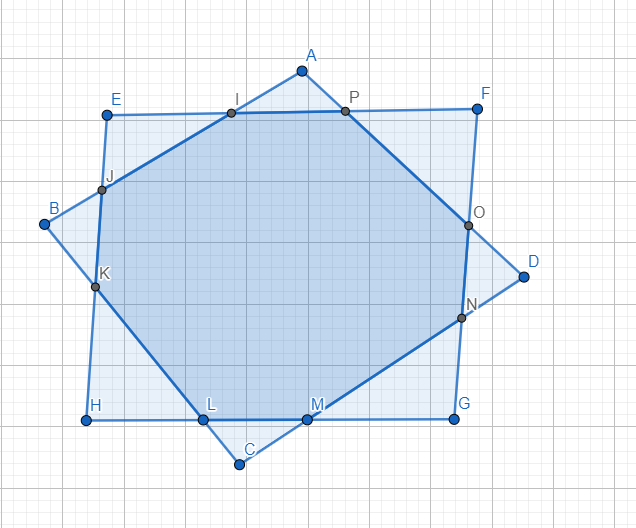
\includegraphics[scale=0.5]{eight_vertices.png} 

I had originally reasoned that having the vertices of $\conv{A}$ on the inside of $\conv{B}$ would give us less points, and same for $\conv{B}$, because it wouldn't let us intersect the edges. This pretty much forces us to take this shape. I believe I have managed to formalize this into a proof, and I think the proof generalizes to any number of dimensions greater than $0$, though with some adjustments after the second.
\end{proof}



In the last problem, we noticed that "protrusions" of intersecting edges gave us the most amount of vertices. Once again, in three dimensions, we can assume that the points are in general position and convex (collinearity and coplanarness would run against what we're trying to do.) In three dimensions, general position and convexness means we have a tetrahedron. We can do something similar by making the faces intersect.\\


Imagine two different tetrahedrons, one representing the convex hull of $A$, the other of $B$. Arrange them so that the vertices of $A$ stick out of exactly one face of $B$, and let them intersect at the faces. Each vertex of $A$ will contribute three vertices for each of the four faces. Hence there are twelve vertices in total.  \\


Actually, we can do even better in turning my mistake into a general solution (and possibly yet more general!!) That being said, my first solution involved squares, where the true analogy in two dimensions would be triangles. This is because a 2-simplex is a triangle, while a 3-simplex is a tetrahedron, and in TDA we learned that a simplex is in fact the convex hull of three vertices in three dimensions, so the problem really does reduce to figuring out how many vertices the intersection between two n-simplices can have.\\


It will be easier to start with the 2-dimensional case. Let's start with a makeshift defintion:

\begin{definition}
Let $P$ and $H$ be convex polygons. We say that a vertex $v$ of $P$ \textbf{contributes} a vertex $u$ of $P\cap H$ if either $v$ is a vertex of $P\cap H$, or if an edge adjacent to $P$ contains a vertex of $P\cap H$. This defines a relation between the vertices in $P$ and those in $P\cap H$, though of course we could have done it the other way around. This relation on it's own won't do the job. A vertex $v$ \textbf{uniquely contributes} a vertex $x$ if there is no other vertex on $P\cap H$ on the line segment $xv$. 
\end{definition}

\begin{lemma}
A vertex of $P$ can contribute at most two vertices two $P\cap H$. 
\end{lemma}
\begin{proof}
There are essentially two cases. 
\end{proof}

\end{proposition}

\section{Problem 1.42}


\begin{definition} Consider any polygon $P$ in $\R^2$. Embed $P$ in $\R^3$. Select a point $v$ such that $v$ is not coplanar with $P$. Denote the vertices of $P$ by $p_1,\dots,p_n$ written in cyclic order. The \textbf{tent} of the point $P$ with the vertex $v$ is the polyhedron formed with faces $vp_1p_2,vp_2p3, ...$ (once again the vertices are writen cyclcically, so it wraps back around).
\end{definition}

\begin{lemma}
Any tent $P$ with $v$ can be tetrahedralized.
\end{lemma}

\begin{proof}
Triangulate $P$. We can now tetrahedralize the tent by extending each triangle out toward $v$. 
\end{proof}

\begin{theorem}
Suppose that we have a polyhedron $P$, such that there is a point $X$ in $P$ so that $X$ us visible to each vertex of $P$. Then $P$ is covered by a vertex at each of it's guards. 
\end{theorem}

\begin{proof}
Draw line segments from each vertex of $P$ to $X$. None of these line segments cross the faces of $P$. Now for each face $F$, we have formed a tent $T(F)$ with $X$ and $F$ as the polygon. The interiors of these tents partition $P$. Moreover, each of these tents can be tetrahedralized, and each of the tetrahedrons shares a vertex of $P$ which covers the entire tetrahedron (since a tetrahedron is a convex region). Hence each tent, for each face, is covered by the vertices of that face. Since the tents union to make up the entire polyhedron, it follows that the vertices of the polyhedron cover the whole thing.
\end{proof}

\begin{definition}
Recall from Topology (Topology Through Inquiry by Francis Su) that a region $R\subset \R^n$ is star-like iff there exists a point $p\in R$ so that the line segment $xp$ is contained within $R$ for all $x$ in $R$. 
\end{definition}

\begin{corollary}
If a polyhedron is star-like, it is covered by a guard placed at each of it's vertices.
\end{corollary}

\begin{lemma}
Let $ABCPQR$ be the Schonhardt polyhedron as shown in the textbook. Let $L$, $M$, $N$ be the midpoints of the edges $AQ$, $BR$, $CP$. Let $X$ be the center (the point of intersection between the midpoints of one line to it's opposite vertex in the triangle) of the triangle $LMN$. Then $X$ is visible by $A,B,C,P,Q,R$. 
\end{lemma}

\begin{proof}

Twist the Schonhardt polyhedron in the direction which the rectangular prism was rotated to form it, so that all of the diagonal edges meet at one point, $X$. Now un-rotate it, and notice that at each point we have a "line of sight" of each of the vertices. Hence each of the vertices can see $X$. 

\end{proof}

\fbox{problem 1.43}

\begin{corollary}
The Schonhardt polyhedron is covered by a guard at each of it's vertices. 
\end{corollary}

\begin{proof}
This follows directly from the last lemma and Theorem 1.
\end{proof}



\section{Exercise 2.3}


\begin{proposition} 
Let $S$ be the four points $\{(0,0),(0,1), (1,0),(1,1)\}\subset \R^2$. Then $\conv(S) =  [1,0]^2$. 
\end{proposition}
\begin{proof}
To show that $\conv(S)\subset [1,0]^2$ it suffices to show that $[1,0]^2$ is a convex set containing $S$. The fact that it contains $S$ is easy, and follows by definition of the set $[0,1]^2$. We need only show that $[0,1]^2$ is convex. Suppose we have points $p_1,p_2\in [0,1]^2$. Then $ p_1 = (x_1,y_1) $ for $x_1\in [0,1]$ and $p_2 = (x_2,y_2)$ for $x_2, y_2\in [0,1]$, as follows by definition of the cartesian product. Now let $p$ be any point on the line between them. From linear algebra, there must exist some $ \alpha,\beta \ge 0$ so that $\alpha + \beta = 1$, and so that $p = (x,y) \alpha p_1 + \beta p_2$. So then $p = (x,y)$ and $ x = \alpha x_1 + \beta x_2$ and $y = \alpha y_1 + \beta y_2$. By closure of posives union zero, we have $x \ge 0$ and $y\ge 0$. We need only show that $x\le 1$ and $y\le 1$. Since $x_1, x_2\le 1$, we have $\alpha + \beta = 1 \ge \alpha x_1 + \beta x_2 = x$, as desired, and similarly for $y$. So both $x,y\in [0,1]$. By definition of the cartesian square, it follows that $p = (x,y)\in [0,1]^2$. Since $p$ was an arbitrary point on the segment $p_1p_2$, it follows that all points on the segment $p_1p_2$ are contained in $[0,1]^2$. Hence $[0,1]^2$ is convex. Having shown that $[0,1]^2$ is a convex set containing $S$, it follows that $\conv{S}\subset [0,1]^2$.\\


Now suppose that we have any point $p$ in $[0,1]^2$. We must show that $ p\in \conv{S}$. By Theorem 2.2 of the textbook, it suffices to construct a convex combination of the points in $S$ equal to $p$.  Conveniently, the points $(1,0),(0,1)$ are the standard basis vectors for $\R^2$ as a vector space. Any point with on $\R^2$ is uniquely expressed as a linear combination of these two vectors. Also notice that another point $(1,1)$ is simply the sum of these two vectors. \\

Since $p\in [0,1]^2$, there are $x,y\in [0,1]$ so that $(x,y) = p$. There are two cases: either $x+y \le 1$ or $x+y > 1$. First suppose that $x+y\le 1$. Also note that by definition of a closed interval, $x,y \ge 0$. Now consider the convex combination 
$$0(0,0) + y(0,1) + x(1,0) + 0(1,1) = (x,y) = p.$$ So in this case, $p$ is a convex combination of the points in $S$, and therefore $p\in \conv{S}$ by Theorem 2.2 of the textbook.\\

Now suppose that $x + y >1$. Then since $0\le x \le 1$ and $0\le y\le 1$, we have $0\le x/2 \le 1/2$ and $0 \le  y/2 \le 1/2$. Hence $ 0 \le \frac{x  + y}{2} \le 1.$ Now consider the convex combination 
$$ 0(0,0) + \frac{y}{2}(0,1) + \frac{y}{2}(1,0) + \frac{x+y}{2}(1,1) = (x,y) = p.$$
In either case, we can express $p$ as a convex combination of the points of $S$. Hence $p\in \conv{S}$ as follows by Theorem 2.2 of the textbook. $p$ was arbitrary in $p$, so it follows that $[0,1]^2 = \conv{S}$.
\end{proof}

\section{Problem 2.4}

\begin{axiom}(Pasch's axiom as it appears in Saunder's Mac Lane's exposition of Hilbert's axioms) If a line meets the segment $AB$ of a triangle $ABC$ and does not contain $C$, then $l$ meets either $AC$ or $BC$. 
\end{axiom}

\begin{theorem}
Let $l_1$ and $l_2$ be distinct lines. Then $l_1$ and $l_2$ intersect at at most one point. 
\end{theorem}

\begin{lemma} (I know I don't have to prove this, but I think I can, and it makes use of what I thought to be useless yet enjoyable reading!) Let $P$ be a triangle, and suppose that $p_4$ is a point not in $P$ such that $p_4$ can see all vertices of $P$. Then there exist $p_1$ and $p_2$ of $P$ such that $p_4p_1p_2$ forms a triangle which contains the other vertex of $P$, which we shall call $p_3$.
\end{lemma}

\begin{proof}
Let $P = p_1p_2p_3$. Suppose $p_4$ is visible to each vertex. In other words, the line segments $p_4p_1$, $p_4p_2$, $p_4p_3$ intersect the boundary of $P$ only at their end-points. Since $p_1p_2p_3$ is a triangle, it's points are not colinear. Hence the lines $l_i = p_4p_i$ for $i = 1,2,3$ are distinct. 
\end{proof}

\begin{proposition}
Let $S$ be a finite point-set on the plane with at least four elements. Then there exists a partition of $S$, $\{A,B\}$, so that $\conv{A}\cap \conv{B} \ne \emptyset$.
\end{proposition}

\begin{proof}

Select any four points $p_1,p_2,p_3,p_4$. Select any three of these four. Without loss of generality, let these be $p_1,p_2,p_3$. Now there are two cases: either $p_1,p_2,p_3$ are colinear or they are not.\\

Suppose first that they are colinear. Then one of the three must be in between the other two (This actually follows from Axiom II.3 of Hilbert's axioms as they appear in the book "Mathematics: Form and Function" by Saunders Mac Lane, so we'd better hope this is true, regardless of our level of hand-wavyness, if geometry is to be what we could call geometry). Without loss of generality, let the between point be $p_2$ ('twould be a crime not to let the between index correspond to the between point!) Then let $'A$ be the set $A' = \{p_1,p_3\}$, and let $B' = \{p_2,p_4\}$. Then clearly $p_2\in \conv{B'}$. Moreover, since $p_2 $ is between the points $p_3$ and $p_1$, both in $A'$, and since $\conv{A'}$ is convex, the point $p_2$ must also be in $\conv{A'}$. Hence $p_2\in \conv{A'}\cap \conv{B'}$, and the set is non-empty.\\

Now suppose that they are not collinear. Then $\conv\{p1,p2,p3\} = P$ forms a triangle. There are two subcases. Either $p_4\in P$ or not. 
\begin{itemize}
\item First suppose that $ p_4\in P $. Then we select $A' = \{p_1,p_2,p_3\}$ and $B' = \{p_4\}$, and $p_4\in \conv{B'}$ and $p_4\in \conv{A'}$.
\item Now suppose that $p_4\not\in P$. Then there are two subsubcases. Either each vertex of $P$ is visibl to $p_4$ or not. 
\begin{itemize}
\item Suppose first that each vertex of $P$ is visible to $p_4$. Certainly then there is one edge of $P$ which is not visible to $p_4$. Select the vertices of this edge, and without loss of generality let them be $p_1,p_2$. Now let $A'' = \{p_1, p_2,p_4\}$. The convex hull containing $A''$ contains also the point $ p_3 $. 
\item Suppose now that not all vertices are visible to $p_4$. Let one such point be $p_3$. Then the line segment $p_4p_3$ must cross the boundary of $P$, and at an edge. Without loss of generality let that edge be $p_1p_2$. Let that point of intersection be $x$. Now let $A'$ be the set $ \{p_3, p_4\} $ and let $B' = \{p_1,p_2\}$ Since the edge $e = p_1p_2$ is the line between points $p_3$ and $p_4$, it follows that the edge $e$ msut be contained within $\conv{B}$, and hence $x\in \conv{B}$. Morever, the set $A''$ must also contain $x$, once again by definition of convexness. 
\end{itemize}
\end{itemize}
\end{proof}

\section{Exercise 2.9}


\begin{proposition}
Let the diameter of a point set $S$ be the largest distance between any two points of $S$. Show that the diameter is achieved by two hull vertices. 
\end{proposition}

\begin{proof}
We have shown that convex hull of a point set is always a convex polygon. Let $p_1$ and $p_2$ be arbitrary points in $S$, and let $P$ be the convex hull of $S$. Consider the line segment between $p_1$ and $p_2$. Draw two lines, $l_1$ and $l_2$, which cross through both $p_1$ and $p_2$ respectively, and which are both perpendicular to the segment $p_1p_2$. It follows then that they are parallel. Recall that the shortest distance between two parallel lines is achieved by any  line segment between them which is perpendicular to both the lines. In fact, I've seen this use as a definition for the distance between parallel lines. Hence $p_1p_2$ represents the shortest possible distance between $l_1$ and $l_2$. \\
 
Suppose now that either one of them (why not $p_1$) is not a vertex of the convex hull $P$. Then there must exist some point other than $p_1$ which lies on $l_1$ or on the side of $l_1$ opposite $p_2$ (otherwise it would be a vertex), and call this vertex $v$.\\ 
 
 
First suppose that $v$ is collinear with $p_1$ and $p_2$. In this case, in order for $v$ to be distinct from $p_1$ (it must be, or else $p_1$ would be a vertex of the hull), it must be the case that $vp_1$ has positive length. Adding this length onto the line segment $p_1p_2$ gives us a longer line: $vp_2$. Hence in this case, $p_1p_2$ cannot represent the greatest distance. \\

Now suppose that $v$ is not collinear. Then the line segment $vp_2$ crosses the line $l_1$ at some point other than $p_1$, call this point $x$ (it may still be the case that $x=v$, in which case we could say that the line segment $vx$ has length zero). Because $xp_2$ crosses through $p_2$, and because at most one parallel line crosses through a point (I think this is a version of the parallel line postulate), we must have $xp_2$ not parallel to $p_1p_2$ (for $p_1p_2$ already crosses through $p_2$). Hence $xp_2$ is not orthogonal to the lines $l_1$ and $l_2$. Hence the length of the line segment $xp_2$ is greater than that of $p_1p_2$. Because $v,x,p_2$ as constructed are collinear, the length of the line segment $vp_2$ is the sum of the lengths of the segment $xp_1$ and $vx$. From this it follows that $p_1p_2$ cannot represent the greatest distance. \\

In either case, a line segment between points in $S$ which has end points which are not vertices to the convex hull $P$ of $S$, cannot represent the diameter o $S$. There are only a finite number of points in $S$. Hence the distances between points in $S$ must also be finite. Because a finite set of real numbers must have a least element, it follows that the diameter is achieved. Because the diameter is achieved, and not by a line segment between points in $S$ which are not vertices, it follows that the diameter is achieved by vertices of the convex hull of $S$. 
\end{proof} 



\end{document}
